\chapter{Application Deployment}
\label{ch:application_deployment}

\section{Introduction}
The ultimate objective of this graduation project is to bridge the gap between academic deep learning research and practical, edge-based clinical utility. This chapter describes the implementation, software architecture, and production deployment of our non-invasive blood glucose estimation system into a fully functional smartphone application. The application provides a user-friendly, real-time interface that allows individuals to capture physiological signals and receive rapid AI-driven metabolic insights on consumer-grade hardware.

\section{App Architecture}
To ensure a high adoption rate and minimize patient anxiety, the interface is designed around principles of minimalist biomedical UI/UX. The application is officially deployed under the system visual identity represented by its production emblem, illustrated in Figure \ref{fig:app_logo}.

\begin{figure}[H]
    \centering
    
\includegraphics[width=0.35\textwidth]{figures/chapter5/logo.png}
    \caption{Official system logo representing the integration of optical arterial pulses with deep learning networks.}
    \label{fig:app_logo}
\end{figure}

The application backend coordinates three primary software layers:
\begin{itemize}
    \item \textbf{Hardware Abstraction Layer (HAL):} Controls the smartphone camera sensor and forces the LED flash to remain open to serve as an optical transillumination source.
    \item \textbf{Signal Processing Pipeline:} Extracts frame-by-frame RGB pixel intensity variances from the fingertip microcirculation to reconstruct the photoplethysmogram (PPG) waveform.
    \item \textbf{Edge Inference Engine:} Runs the optimized, lightweight 1D-ResNet model locally to convert the captured temporal time-series signal into a precise blood glucose regression value.
\end{itemize}

\section{Live Signal Monitor}
When a user initializes the measurement sequence, the application activates the smartphone camera. The patient is instructed to cover the camera lens and LED flash entirely with their index finger. 

As shown in Figure \ref{fig:ppg_live}, before data logging begins, the application renders a dynamic, live visual feedback loop displaying the real-time heart rate (BPM) alongside a micro-graphical presentation of the incoming raw cardiac pulse wave. A localized signal quality estimator evaluates the input metrics, providing a ``Signal: Good'' structural status to ensure correct finger placement and uniform illumination before the user triggers the definitive recording stage.

\begin{figure}[H]
    \centering
    
\includegraphics[width=0.42\textwidth]{figures/chapter5/ppg_live_monitor.png.png}
    \caption{The real-time pre-measurement interface displaying initial BPM and live optical waveform status.}
    \label{fig:ppg_live}
\end{figure}

\section{Data Acquisition}
Upon clicking the engagement control, the interface transitions into an active logging state, as illustrated in Figure \ref{fig:recording_ppg}. The system collects continuous raw optical data over a fixed temporal window required by the underlying 1D-ResNet regression matrix. A progressive linear status bar tracks the elapsed acquisition period, while the underlying engine continuously updates the localized vital statistics and verifies signal stability. Users can abort the routine at any point by engaging the prominent ``Stop Recording'' safety override.

\begin{figure}[H]
    \centering
    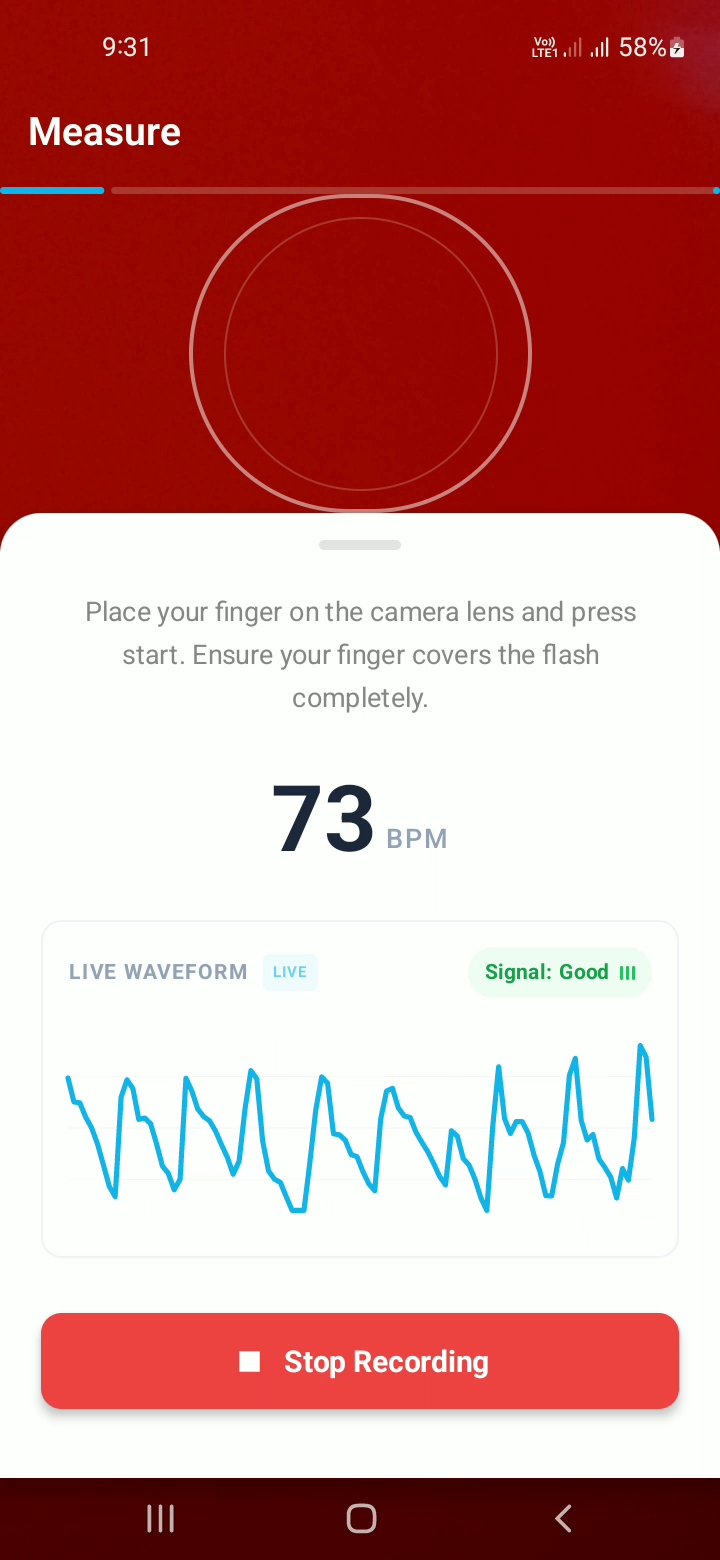
\includegraphics[width=0.42\textwidth]{figures/chapter5/recording_ppg.png}
    \caption{Active data collection interface capturing continuous raw PPG wave arrays over a fixed duration.}
    \label{fig:recording_ppg}
\end{figure}

\section{AI Inference}
Once the signal window is completely captured and isolated, the application packages the raw time-series array and pushes it to the localized deep learning execution block. Figure \ref{fig:loading_analysis} demonstrates the interim processing state during which the background thread normalizes the incoming waveform, isolates motion artifacts via baseline filters, and feeds the streamlined signal matrix through the compressed convolutional layers of our fine-tuned network.

\begin{figure}[H]
    \centering
    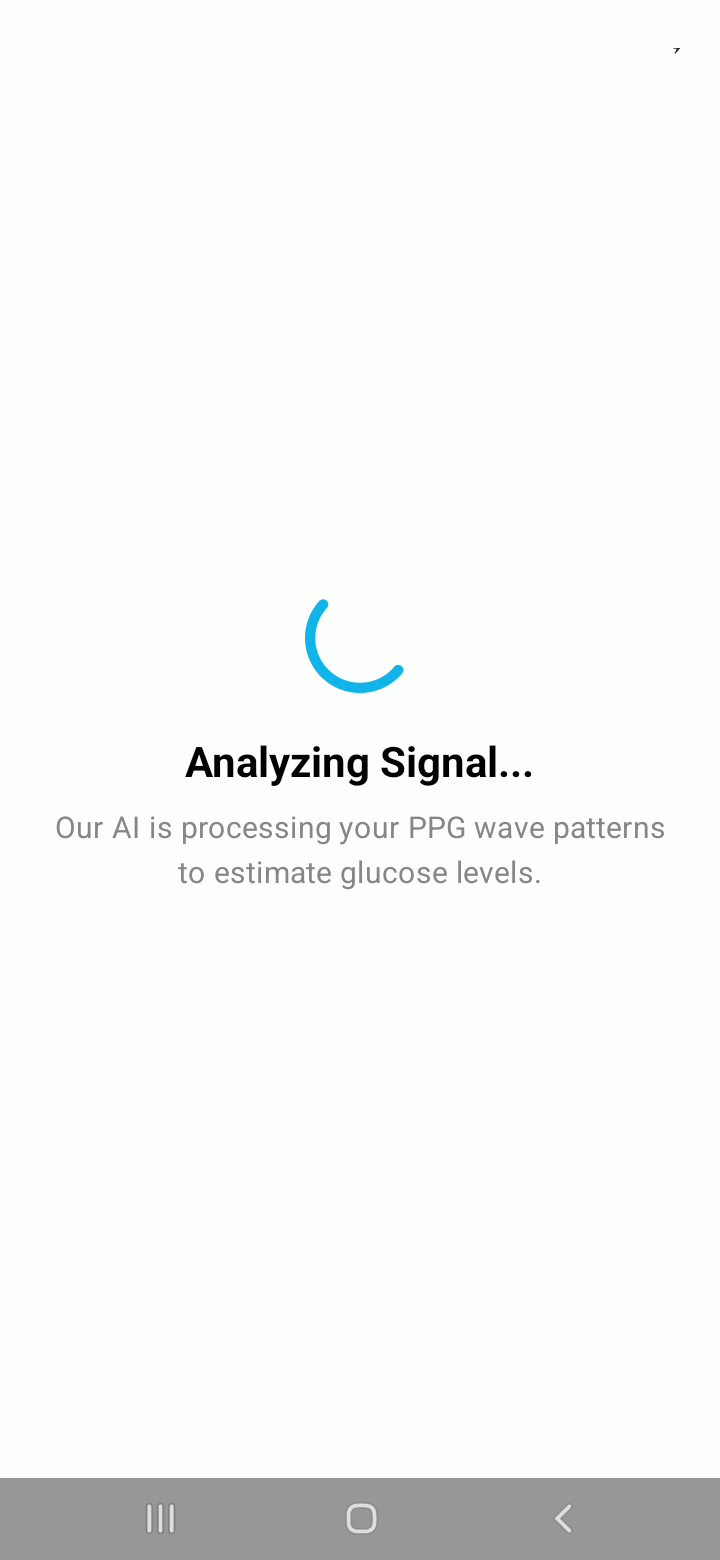
\includegraphics[width=0.42\textwidth]{figures/chapter5/loading_ai_analysis.png}
    \caption{Interim localized deep learning analysis layer performing signal normalization and 1D-ResNet execution.}
    \label{fig:loading_analysis}
\end{figure}

\section{Result Presentation}
The output of the mathematical regression model is immediately delivered to the final presentation layer, shown in Figure \ref{fig:glucose_result}. The screen provides clear verification of a successful cycle via a centralized confirmation emblem, accompanied by the primary clinical metric displaying the estimated blood glucose concentration calibrated in milligrams per deciliter ($\text{mg/dL}$). 

\begin{figure}[H]
    \centering
    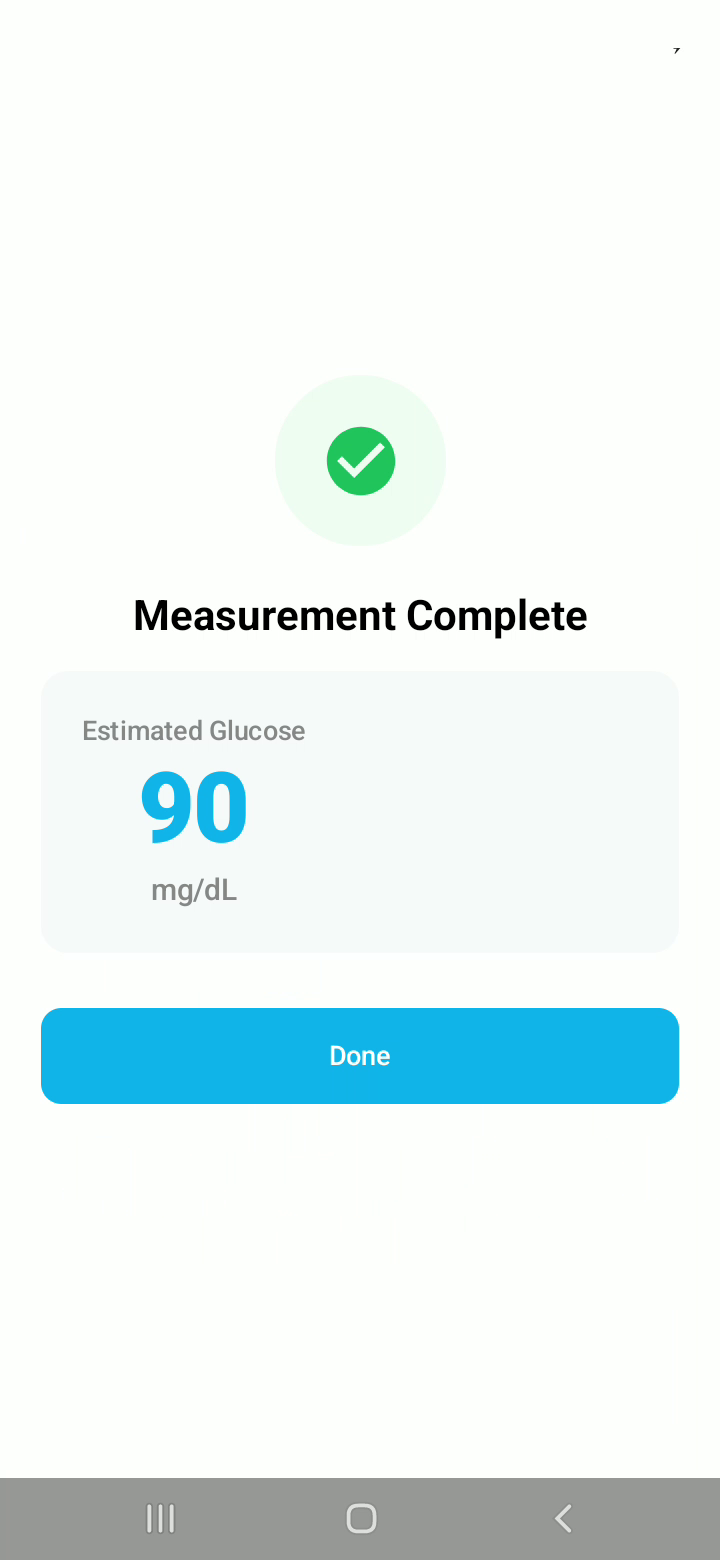
\includegraphics[width=0.42\textwidth]{figures/chapter5/ai_glucose_result.png}
    \caption{Final measurement presentation screen demonstrating a non-invasive estimation output of 90 mg/dL.}
    \label{fig:glucose_result}
\end{figure}

By hitting the final ``Done'' trigger, the temporary memory stack is safely cleared, and the application returns to its initial standby position, ready for subsequent real-time diagnostic sessions. This complete deployment achieves the project's engineering goal of delivering an instantaneous, painless, and highly accessible consumer health tool.